\subsection{OTFS Transmitter Design}

\subsubsection{Overview of the Transmitter Processing Chain}

The OTFS transmitter is designed to convert a binary information sequence into a time-domain waveform suitable for transmission over a time-varying multipath channel. The key idea is that the information symbols are first arranged in the delay-Doppler domain, rather than being transmitted directly in the time-frequency domain. This processing structure allows the transmitted frame to be associated with the delay and Doppler characteristics of the wireless channel.

The overall transmitter chain used in the baseline OTFS system is illustrated in Fig.~\ref{fig:otfs_transmitter_chain}. The input bit sequence is first mapped into QAM symbols. These symbols are then placed on the delay-Doppler grid to form the matrix \(\mathbf{x}_{\mathrm{DD}}\). After that, the inverse symplectic finite Fourier transform is applied to convert the delay-Doppler symbols into the time-frequency domain. The resulting time-frequency symbols are finally transformed into a time-domain transmit signal by the Heisenberg transform, or equivalently by its discrete implementation in the simulation.

\begin{figure}[H]
    \centering
    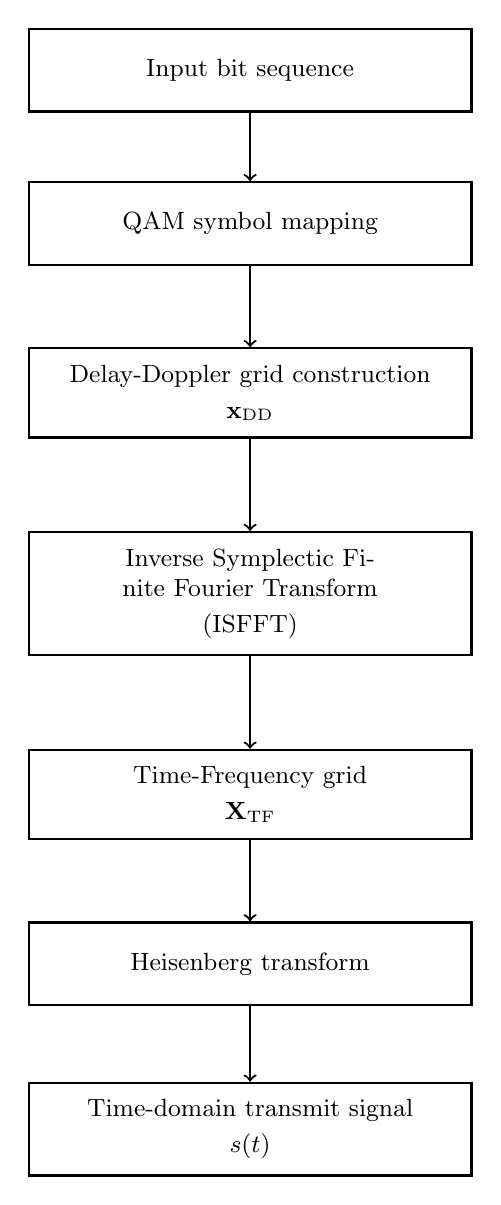
\begin{tikzpicture}[
        block/.style={
            rectangle,
            draw,
            thick,
            align=center,
            text width=5.2cm,
            minimum height=1.05cm,
            font=\small,
            inner sep=6pt
        },
        arrow/.style={
            ->,
            thick,
            shorten >=0pt,
            shorten <=0pt
        }
    ]

        \node[block] (bits) at (0,0) {Input bit sequence};
        \node[block] (qam) at (0,-1.95) {QAM symbol mapping};
        \node[block] (dd) at (0,-4.10) {Delay-Doppler grid construction\\[2pt]\(\mathbf{x}_{\mathrm{DD}}\)};
        \node[block] (isfft) at (0,-6.65) {Inverse Symplectic Finite Fourier Transform\\[2pt](ISFFT)};
        \node[block] (tf) at (0,-9.20) {Time-Frequency grid\\[2pt]\(\mathbf{X}_{\mathrm{TF}}\)};
        \node[block] (heis) at (0,-11.35) {Heisenberg transform};
        \node[block] (tx) at (0,-13.45) {Time-domain transmit signal\\[2pt]\(s(t)\)};

        \draw[arrow] (bits.south) -- (qam.north);
        \draw[arrow] (qam.south) -- (dd.north);
        \draw[arrow] (dd.south) -- (isfft.north);
        \draw[arrow] (isfft.south) -- (tf.north);
        \draw[arrow] (tf.south) -- (heis.north);
        \draw[arrow] (heis.south) -- (tx.north);

    \end{tikzpicture}
    \caption{Baseline OTFS transmitter processing chain}
    \label{fig:otfs_transmitter_chain}
\end{figure}

The transmitter can therefore be viewed as a sequence of four main operations. The first operation is bit-to-symbol mapping, where the input bits are grouped and mapped to QAM constellation points. The second operation is delay-Doppler grid construction, where the QAM symbols are arranged over the \(N \times M\) OTFS frame. The third operation is the inverse symplectic finite Fourier transform, which maps the delay-Doppler representation to the time-frequency representation. The final operation is time-domain signal generation, where the time-frequency samples are converted into the transmitted waveform.

This separation of operations is useful because each stage has a distinct role in the OTFS system. The QAM mapper determines the number of bits carried by each active resource element. The delay-Doppler grid defines the information-bearing structure of the OTFS frame. The ISFFT performs the domain transformation required by OTFS modulation, while the Heisenberg transform generates the signal that is actually transmitted through the channel. In the baseline OTFS system, all delay-Doppler grid positions are active, which makes the transmitter structure simpler than the OTFS-IM transmitter introduced in Chapter 4.

In the discrete simulation model, the transmitter follows the same conceptual chain. A random bit sequence is generated and mapped to 4-QAM symbols. The symbol vector is reshaped into an \(N \times M\) delay-Doppler matrix. The OTFS modulation stage then performs the discrete transform operations and serializes the result into a time-domain vector. This vector is used as the input to the multipath delay-Doppler channel model described in the next section.

\subsubsection{Bit-to-QAM Symbol Mapping}

The first stage of the baseline OTFS transmitter is the mapping of information bits to QAM symbols. In the OTFS notation used in this thesis, the information symbols before modulation are denoted by \(x[k,l]\), where \(k\) is the Doppler index and \(l\) is the delay index. These symbols form the delay-Doppler information grid that will later be transformed into the time-frequency domain.

For one OTFS frame, the transmitter generates a binary information sequence with
\begin{equation}
    B_{\mathrm{OTFS}} = MN\log_2(M_{\mathrm{QAM}})
\end{equation}
bits, where \(M_{\mathrm{QAM}}\) is the QAM modulation order. For the baseline setup, \(N=10\), \(M=12\), and \(M_{\mathrm{QAM}}=4\), so one OTFS frame contains
\begin{equation}
    B_{\mathrm{OTFS}} = 10 \times 12 \times \log_2(4) = 240
\end{equation}
information bits.

The input bit sequence is divided into groups of \(\log_2(M_{\mathrm{QAM}})\) bits. Each group is converted into a decimal symbol index and then mapped to one QAM constellation point. This produces a vector of \(MN\) complex-valued QAM symbols. This mapping is represented by
\begin{equation}
    \mathbf{x}
    =
    \mathcal{Q}_{M_{\mathrm{QAM}}}
    \left(
    \mathbf{b}
    \right),
\end{equation}
where \(\mathcal{Q}_{M_{\mathrm{QAM}}}(\cdot)\) denotes grouping the input bits and mapping each group to an \(M_{\mathrm{QAM}}\)-ary QAM constellation point.

After QAM mapping, the symbol vector is reshaped into the delay-Doppler grid as
\begin{equation}
    \mathbf{x}_{\mathrm{DD}}
    =
    \left[
    x[k,l]
    \right]_{N \times M}.
\end{equation}
In the code, this step is performed by
\begin{equation}
    \mathbf{x}_{\mathrm{DD}}
    =
    \mathrm{reshape}(\mathbf{x},N,M).
\end{equation}

For the baseline OTFS system, all positions on the delay-Doppler grid are active. Therefore, every element \(x[k,l]\) carries one QAM symbol. This is an important difference from the OTFS-IM transmitter introduced in Chapter 4, where only selected positions are active and the active-position pattern itself also conveys information.

With 4-QAM modulation, each delay-Doppler resource element carries two information bits. Therefore, the baseline OTFS transmitter maps the 240 input bits of one frame into 120 QAM symbols and places them over the full \(10 \times 12\) delay-Doppler grid. The resulting matrix \(\mathbf{x}_{\mathrm{DD}}\) is then used as the input to the OTFS modulation block.

\subsubsection{Delay-Doppler Grid Construction}

After QAM symbol mapping, the next stage is to arrange the modulated symbols onto the OTFS delay-Doppler grid. This grid is the information-bearing domain of OTFS. Instead of assigning symbols directly to time-frequency resource elements as in OFDM, OTFS first places the QAM symbols in the delay-Doppler domain. The subsequent OTFS modulation stages then spread these symbols over the time-frequency plane before transmission.

Let the QAM symbol vector generated by the previous stage be denoted by
\begin{equation}
    \mathbf{x}
    =
    [x_0,x_1,\ldots,x_{MN-1}]^T.
\end{equation}
This vector contains \(MN\) complex-valued QAM symbols. In the baseline OTFS transmitter, these symbols are reshaped into the delay-Doppler symbol matrix
\begin{equation}
    \mathbf{x}_{\mathrm{DD}}
    =
    [x[k,l]]
    \in \mathbb{C}^{N \times M},
\end{equation}
where \(k=0,1,\ldots,N-1\) denotes the Doppler index and \(l=0,1,\ldots,M-1\) denotes the delay index.

The mapping from the one-dimensional QAM symbol vector to the two-dimensional delay-Doppler grid can be written as
\begin{equation}
    x[k,l] = x_{k + lN},
    \qquad
    0 \leq k \leq N-1,\quad 0 \leq l \leq M-1.
\end{equation}
This indexing follows a fixed column-wise ordering when the one-dimensional symbol sequence is arranged into the \(N \times M\) delay-Doppler grid. Equivalently, the reshaping operation can be represented as
\begin{equation}
    \mathbf{x}_{\mathrm{DD}}
    =
    \mathrm{reshape}(\mathbf{x},N,M).
\end{equation}

For the baseline OTFS system, every position of the delay-Doppler grid is occupied by one QAM symbol. Therefore, the grid contains no inactive resource elements. This full-grid structure is important because it defines the conventional OTFS reference system. In Chapter 4, the OTFS-IM transmitter modifies this structure by dividing the grid into index-modulation blocks and activating only selected positions inside each block.

For the simulation configuration used in this thesis, the grid size is \(N=10\) and \(M=12\). Hence, the delay-Doppler grid contains \(120\) symbol positions. With 4-QAM modulation, the transmitter maps \(240\) input bits into \(120\) QAM symbols and places them over the full delay-Doppler grid. The resulting matrix \(\mathbf{x}_{\mathrm{DD}}\) is then used as the input to the inverse symplectic finite Fourier transform in the next stage of the OTFS modulator.

A conceptual view of the baseline delay-Doppler grid is shown in Fig.~\ref{fig:baseline_dd_grid}. Each cell represents one delay-Doppler resource element, and all cells are active in the baseline OTFS system.

\begin{figure}[H]
    \centering
    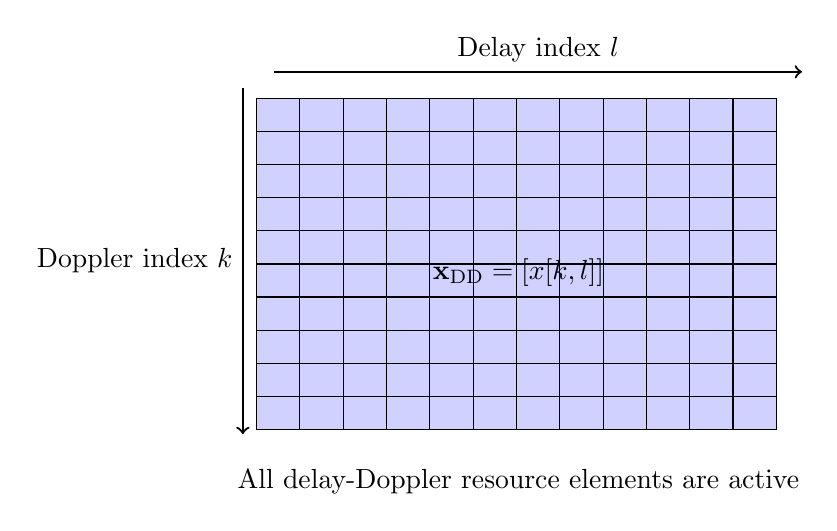
\begin{tikzpicture}[
        cell/.style={
            rectangle,
            draw,
            minimum width=0.55cm,
            minimum height=0.42cm
        },
        active/.style={
            fill=blue!18
        }
    ]

        \foreach \i in {0,...,9} {
            \foreach \j in {0,...,11} {
                \node[cell, active] at (\j*0.55,-\i*0.42) {};
            }
        }

        \draw[->, thick] (-0.45,0.35) -- (-0.45,-4.05)
            node[midway, left] {Doppler index \(k\)};
        \draw[->, thick] (-0.05,0.55) -- (6.65,0.55)
            node[midway, above] {Delay index \(l\)};

        \node at (3.05,-2.0) {\(\mathbf{x}_{\mathrm{DD}}=[x[k,l]]\)};
        \node[align=center] at (3.05,-4.65) {All delay-Doppler resource elements are active};

    \end{tikzpicture}
    \caption{Baseline OTFS delay-Doppler grid with full resource activation}
    \label{fig:baseline_dd_grid}
\end{figure}

\subsubsection{Inverse Symplectic Finite Fourier Transform}

After the QAM symbols are arranged on the delay-Doppler grid, the next step of the OTFS transmitter is to transform them into the time-frequency domain. This operation is performed by the inverse symplectic finite Fourier transform. The ISFFT is one of the core operations of OTFS modulation because it connects the information-bearing delay-Doppler representation to the time-frequency representation used for waveform generation.

Let the delay-Doppler symbol matrix be denoted by
\begin{equation}
    \mathbf{x}_{\mathrm{DD}} = [x[k,l]],
\end{equation}
where \(k=0,1,\ldots,N-1\) is the Doppler index and \(l=0,1,\ldots,M-1\) is the delay index. The ISFFT maps \(x[k,l]\) into the time-frequency symbols \(X[n,m]\), where \(n=0,1,\ldots,N-1\) denotes the time index and \(m=0,1,\ldots,M-1\) denotes the frequency index.

Using the OTFS convention adopted in this thesis, the ISFFT can be written as
\begin{equation}
    X[n,m]
    =
    \frac{1}{\sqrt{MN}}
    \sum_{k=0}^{N-1}
    \sum_{l=0}^{M-1}
    x[k,l]
    e^{j2\pi\left(\frac{nk}{N}-\frac{ml}{M}\right)}.
    \label{eq:isfft}
\end{equation}
The resulting matrix
\begin{equation}
    \mathbf{X}_{\mathrm{TF}}
    =
    [X[n,m]]
    \in \mathbb{C}^{N \times M}
\end{equation}
represents the OTFS frame in the time-frequency domain.

The structure of the ISFFT is different from a conventional two-dimensional inverse Fourier transform because the signs of the Fourier kernels are opposite along the two dimensions. This symplectic structure reflects the dual relationship between the delay-Doppler and time-frequency domains. In particular, the Doppler dimension is transformed with respect to the time index, while the delay dimension is transformed with respect to the frequency index.

For the discrete implementation used in the simulation model, the ISFFT operation is evaluated through a pair of finite Fourier transforms along the two grid dimensions:
\begin{equation}
    \mathbf{X}_{\mathrm{TF}}
    =
    \mathrm{fft}
    \left(
    \mathrm{ifft}
    \left(
    \mathbf{x}_{\mathrm{DD}}
    \right)^T
    \right)^T
    \bigg/
    \sqrt{\frac{M}{N}}.
    \label{eq:isfft_matlab}
\end{equation}
This expression is the matrix-form counterpart of the ISFFT in \eqref{eq:isfft}. The two transform directions correspond to the delay and Doppler dimensions, while the normalization factor preserves the energy scale of the OTFS frame.

The normalization factor is included to preserve the signal energy across the domain transformation. This is important for BER simulation because the noise variance is computed from the selected \(E_b/N_0\) value. If the transform scaling were inconsistent, the effective received SNR would be shifted, making the BER comparison between OFDM, OTFS, and OTFS-IM unfair.

After the ISFFT, each delay-Doppler information symbol has been spread across the time-frequency grid. This spreading property is one of the reasons OTFS is suitable for time-varying multipath channels. Instead of assigning each information symbol to a single time-frequency resource element, OTFS distributes the symbol over the frame before waveform generation. The time-frequency matrix \(\mathbf{X}_{\mathrm{TF}}\) is then passed to the Heisenberg transform to generate the time-domain transmit signal.

\subsubsection{Heisenberg Transform and Time-Domain Signal Generation}

After the ISFFT, the OTFS frame is represented by the time-frequency symbol matrix
\begin{equation}
    \mathbf{X}_{\mathrm{TF}} = [X[n,m]],
\end{equation}
where \(n=0,1,\ldots,N-1\) is the time index and \(m=0,1,\ldots,M-1\) is the frequency index. The purpose of the Heisenberg transform is to convert these time-frequency samples into a continuous-time transmit waveform.

In the general OTFS formulation, the transmitted signal can be expressed as
\begin{equation}
    s(t)
    =
    \sum_{n=0}^{N-1}
    \sum_{m=0}^{M-1}
    X[n,m]\,
    g_{\mathrm{tx}}(t-nT)
    e^{j2\pi m\Delta f(t-nT)},
    \label{eq:heisenberg_transform}
\end{equation}
where \(g_{\mathrm{tx}}(t)\) is the transmit pulse, \(T\) is the symbol duration, and \(\Delta f\) is the subcarrier spacing. This expression shows that each time-frequency sample \(X[n,m]\) modulates a time-shifted and frequency-shifted version of the transmit pulse.

The Heisenberg transform can be viewed as the waveform-generation stage of the OTFS transmitter. While the delay-Doppler grid defines where the information symbols are placed, and the ISFFT maps them into the time-frequency domain, the Heisenberg transform produces the actual signal that enters the wireless channel. Therefore, it plays a role similar to the multicarrier modulation stage in OFDM, but it operates on the time-frequency samples generated from the delay-Doppler information grid.

In the discrete model used in this thesis, the Heisenberg transform is represented after the ISFFT by applying an inverse Fourier transform along the frequency-related dimension:
\begin{equation}
    \mathbf{s}_{\mathrm{mat}}
    =
    \mathrm{ifft}
    \left(
    \mathbf{X}_{\mathrm{TF}}^T
    \right)
    \sqrt{M}.
    \label{eq:heisenberg_matlab}
\end{equation}
This matrix \(\mathbf{s}_{\mathrm{mat}}\) contains the time-domain samples associated with the time-frequency grid \(\mathbf{X}_{\mathrm{TF}}\). The scaling factor keeps the discrete waveform normalization consistent with the ISFFT stage.

The matrix \(\mathbf{s}_{\mathrm{mat}}\) contains the discrete time-domain samples before serialization. To form the transmit vector, the matrix is converted into a column vector according to
\begin{equation}
    \mathbf{s}
    =
    \mathrm{vec}
    \left(
    \mathbf{s}_{\mathrm{mat}}
    \right).
    \label{eq:tx_vector}
\end{equation}
The vectorization step preserves the sample ordering used by the OTFS frame and produces a one-dimensional transmit sequence suitable for the channel model.

The output vector \(\mathbf{s}\) is the discrete-time transmit signal used as the input to the wireless channel model. In the simulation framework, this signal is passed to the time-varying multipath channel model, where delay taps, Doppler taps, fading coefficients, and additive noise are applied. Therefore, the Heisenberg transform and serialization stage completes the baseline OTFS transmitter processing chain.

\subsubsection{Discrete Processing Summary}

The baseline OTFS transmitter can be summarized by three discrete signal-processing operations: ISFFT, discrete Heisenberg transformation, and serialization. The input is the delay-Doppler matrix \(\mathbf{x}_{\mathrm{DD}}\), obtained by arranging the QAM symbol vector according to the \(N \times M\) frame ordering described earlier. The output is the time-domain transmit vector \(\mathbf{s}\).

The complete discrete transmitter chain can therefore be summarized as
\begin{equation}
\begin{aligned}
    \mathbf{X}_{\mathrm{TF}}
    &=
    \mathrm{fft}
    \left(
    \mathrm{ifft}
    \left(
    \mathbf{x}_{\mathrm{DD}}
    \right)^T
    \right)^T
    \bigg/
    \sqrt{\frac{M}{N}},
    \\
    \mathbf{s}_{\mathrm{mat}}
    &=
    \mathrm{ifft}
    \left(
    \mathbf{X}_{\mathrm{TF}}^T
    \right)
    \sqrt{M},
    \\
    \mathbf{s}
    &=
    \mathrm{vec}
    \left(
    \mathbf{s}_{\mathrm{mat}}
    \right).
\end{aligned}
\end{equation}

This compact representation is important for the rest of the thesis because the same OTFS modulation principle is used for both the baseline OTFS system and the later OTFS-IM system. The difference between the two systems is not in the modulation transform itself, but in the construction of the delay-Doppler input matrix. In the baseline OTFS system, every delay-Doppler position carries a QAM symbol, while in OTFS-IM only selected positions are active according to an index-modulation pattern.

\subsubsection{Summary of the Baseline OTFS Transmitter}

The baseline OTFS transmitter converts a binary information sequence into a time-domain signal through a sequence of delay-Doppler and time-frequency processing stages. The input bits are first mapped to QAM symbols and arranged on the delay-Doppler grid as \(x[k,l]\). In the baseline system, all delay-Doppler resource elements are active, so every grid position carries one QAM symbol.

The delay-Doppler symbol matrix \(\mathbf{x}_{\mathrm{DD}}\) is then transformed into the time-frequency domain by the ISFFT. This produces the time-frequency matrix \(\mathbf{X}_{\mathrm{TF}}\), whose elements \(X[n,m]\) are used for waveform generation. The discrete Heisenberg transform is finally applied to obtain the time-domain transmit vector \(\mathbf{s}\).

The transmitter chain can be summarized as
\begin{equation}
    \mathbf{b}
    \rightarrow
    \mathbf{x}
    \rightarrow
    \mathbf{x}_{\mathrm{DD}}
    \xrightarrow{\mathrm{ISFFT}}
    \mathbf{X}_{\mathrm{TF}}
    \xrightarrow{\mathrm{Heisenberg}}
    \mathbf{s}.
\end{equation}

This structure highlights the main difference between OTFS and conventional OFDM. In OFDM, information symbols are directly assigned to time-frequency resource elements. In OTFS, the information symbols are first placed in the delay-Doppler domain and then spread across the time-frequency plane before transmission. This spreading allows the transmitted frame to interact with the delay-Doppler structure of the wireless channel.

The same OTFS modulation block is reused later for the OTFS-IM transmitter. The key difference is the construction of the delay-Doppler input matrix. In the baseline OTFS system, every grid position is active. In OTFS-IM, only selected positions are active, and their indices carry additional information bits. Therefore, the baseline transmitter developed in this section provides the foundation for the OTFS-IM design in Chapter 4.

After the time-domain signal \(\mathbf{s}\) is generated, it is passed through the time-varying multipath channel. The design of this channel model and its delay-Doppler characteristics are discussed in the next section.
